\chapter{Tervezés}
\label{cha:design}

Ahogy a \ref{cha:osgi}.~fejezetben is láttuk az OSGi keretrendszer megfelel a kiírásban specifikált szoftver által támasztott követelményeknek, felhasználásával a rendszer kellően flexibilis lesz. Az \ref{cha:related_work}.~fejezetben levont tanulságok alapján érdemes megtervezni a rendszert, illetve az ott említett Wikipédia Miner architektúráját fel lehet használni a tervezés során, az alapvető komponensek meghatározásában segíthet.

Első lépésként meghatároztam a leendő rendszer komponenseit (\ref{fig:componentdiagram}.~ábra), mely képes folyamatosan működve a Wikipédia tartalmát rendszerezett formában eltárolni és azt később a rá épülő alkalmazások számára elérhetővé tenni. Mivel a rendszer első indításakor az adatbázisban még semmilyen adatok nem találhatóak, és a Wikipédia frissülő cikkeinek követésével, csak az aktuális változások kerülnek be az adatbázisba, a rendszer indításakor már a Wikipédián korábban közzétett cikkek nem kerülnek be a felépített tudásbázisba. Ezt a problémát úgy lehet a legegyszerűbben megoldani, hogy az on-the-fly feldolgozás mellett a statikus dumpból való adatok importálását is lehetővé tesszük. Ezzel kombináljuk a \ref{cha:related_work}.~fejezetben megismert alkalmazások előnyét a követelményekben meghatározottakkal, így egy sokkal erősebb eszköz állítható elő.

\begin{figure}[htp]
\centering
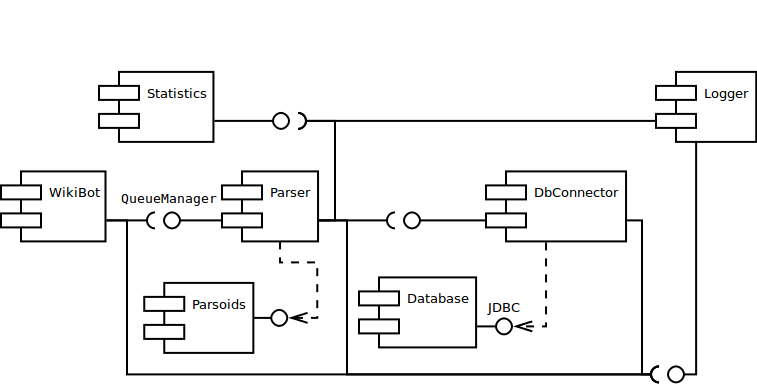
\includegraphics[scale=0.5]{img/componentdiagram}
\caption{Az alkalmazás tervezett komponensei}
\label{fig:componentdiagram}
\end{figure}

A követelményekből következően szükségszerűen meghatározott komponenseken túl az alkalmazás minőségének javítása érdekében érdemes a komponensek felügyelhetőségét is biztosítani. Ezáltal az alkalmazás működéséből részletesebb adatok is megfigyelhetővé válnak azon kívül, hogy működik vagy sem a rendszer, illetve a funkcionalitás tesztelése és a teljesítménymérés is sokkal egyszerűbb lesz. A felügyelhetőséget naplózás és különféle metrikák segítségével terveztem lehetővé tenni.

Miután a különálló komponenseket meghatároztam, megkezdődhetett sorban az egyes komponensek megtervezése. Minden komponenst a komponensalapú fejlesztésnek megfelelően egyesével, mint különálló programokat lehetett megtervezni és implementálni. A következőkben bemutatom az egyes komponensek szerepét, alapvető működését és a tervezésük lépéseit.

\section{WikiBot bundle}
\label{sec:wikibotbundle}

Az adatok on-the-fly feldolgozásáért felelős ez a komponens. Ezt a tulajdonságot a frissülő cikkek megszerzésének módjával fogom biztosítani. Az adatok könnyű kezelése miatt minden cikknek egy reprezentációját is ki kell alakítani a programban, amelyet tovább kell adni a következő komponensek számára, további feldolgozás céljából. Ezek alapján meghatározott use-case-ek láthatóak a \ref{fig:usecase_wikiBot}.~ábrán.

\begin{figure}[htp]
\centering
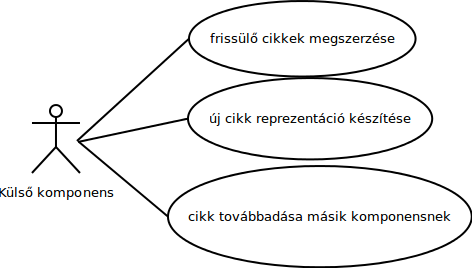
\includegraphics[scale=0.6]{img/usecase_wikiBot}
\caption{A WikiBot komponens használati esetei}
\label{fig:usecase_wikiBot}
\end{figure}

Megtervezését egy rövidebb előkutatás előzte meg, mely során keresni kellett valamilyen lehetőséget, amelynek segítségével folyamatosan értesülhet az alkalmazás, ha egy új Wikipédia cikk jelenik meg, vagy frissítenek egyet a hivatalos oldalon. A legegyszerűbb megoldásnak végül a hivatalos, Wikipédia által üzemeltett IRC csatorna tűnt, ahol folyamatosan publikálják az oldalon frissülő cikkeket.

\begin{figure}[htp]
\centering
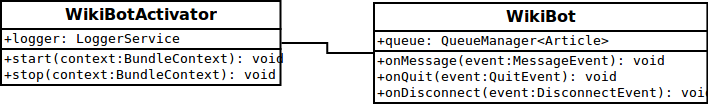
\includegraphics[scale=0.55]{img/class_wikiBot}
\caption{A tervezett WikiBot osztálydiagramja}
\label{fig:class_wikiBot}
\end{figure}

A tervezett komponens tehát egy IRC Bot kliens lesz, amely a fent említett IRC csatornára lesz feliratkozva. A tervezésnél figyelni kellett arra, hogy miután megszerzi az új cikk szükséges adatait, azokat azonnal tovább kell adnia a következő komponensnek. Más teendőket nem végezhet, működését nem szabad hosszú távon feltartani, mert a gyorsan frissülő cikkek miatt elvesznek az IRC csatorna által küldött információk, míg a komponens mással foglalkozik.

A komponens két osztályból fog állni, az egyik egy OSGi BundleActivator implementáció (\texttt{WikiBotActivator} osztály), mely menedzseli a komponens indulását, leállítását, a másik pedig a Wikipédia IRC csatornájával való kommunikációt kezeli (\texttt{WikiBot}).

A tervezett működés szerint a rendszer a \texttt{WikiBotActivator} elindulásával kezdődik, melyet az OSGi keretrendszer példányosít számunkra, majd elindítja azt. A lehető leggyorsabb működés úgy érhető el, hogy ne tartsuk fel a komponens működését, ha az új cikk megszerzett adatait eltároljuk egy átmeneti tárolóban (\texttt{QueueManager} osztály). Ez a queue, ahogy a \ref{fig:componentdiagram}.~ábrán is látható a Parser komponens egy kiajánlott OSGi szolgáltatása. A \texttt{QueueManager} osztály bemutatása a \ref{sec:parserbundle} alfejezetben folytatódik. A kiajánlott queue referenciáját az OSGi \texttt{BundleContext}-en keresztül lehet majd megszerezni.

Továbbiakban a \texttt{WikiBot} belép a Wikipédia egyik IRC szobájába, ahol az angol nyelvű cikkeket teszik közzé. Az implementált IRC Bot-ban egy eseménykezelőt kell megvalósítani (\texttt{.onMessage()} metódus), ami akkor hívódik meg, ha egy új üzenet érkezik az IRC szobába. Egy példa üzenet figyelhető meg a \ref{lst:ircexample}.~kódrészletben.

\begin{lstlisting}[label={lst:ircexample}, caption=Példa üzenet az angol nyelvű Wikipédia IRC csatornájából,breaklines=true]
(11.16.43) rc-pmtpa: [[History of Vietnam]]  http://en.wikipedia.org/w/index.php?diff=580135314&oldid=580104406 * 124.170.231.126 * (+95) 
\end{lstlisting}

Minden egyes beérkezett üzenet alapján egy új cikk reprezentációt (\texttt{Article} osztály) hoz létre, mely később végig fog haladni a teljes feldolgozóláncon. A szükséges adatok a cikk címe, mely dupla szögletes zárójelek között található, valamint az új cikk verziószáma, mely az üzenetben található link \texttt{diff} GET paraméterében található. Végül az összeállított cikket a korábban megszerzett \texttt{QueueManager}-ben helyezi el.

Az alapvető követelményeken felül a megfigyelhetőséget is érdemes biztosítani, amelyet a \texttt{WikiBot} komponensnél naplózással oldottam meg. A \texttt{WikiBotActivator} indulásakor a \texttt{Logger} komponens (\ref{sec:loggerbundle}.~alfejezet) referenciáját is megszerzi, melyet naplózásra használhat.

% section wikibotbundle (end)

\section{Parser bundle}
\label{sec:parserbundle}

Ebben a komponensben kell lennie valamilyen tároló elemnek, egyfajta queue megoldásnak, melynek szükségessét az előző \ref{sec:wikibotbundle}.~alfejezetben fejtettem ki. Ennek a queue megoldásnak szálbiztosnak kell lennie, hiszen egyszerre fog a WikiBot és a Parser komponens dolgozni vele, ezenkívül a tárolónak blokkolnia is kell beszúrást, ha már túl sok elem van benne. A módosult, vagy újonnan létrehozott cikkek szövegét meg kell szereznie a komponensnek, majd azt át kell alakítania egy meghatározott formátumra. Végül a cikket tovább kell adnia egy másik komponensnek eltárolás céljából. Ezek alapján készíthető el a a use-case diagram (\ref{fig:usecase_parser}.~ábra).

\begin{figure}[htp]
\centering
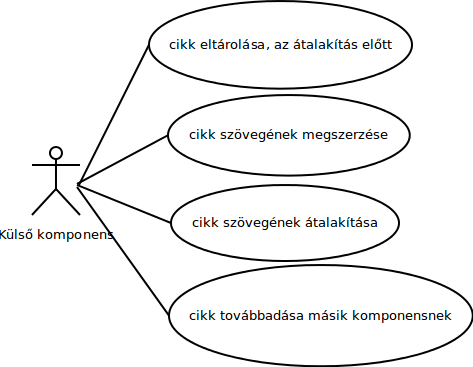
\includegraphics[scale=0.6]{img/usecase_parser}
\caption{A Parser komponens használati esetei}
\label{fig:usecase_parser}
\end{figure}

Ahhoz, hogy egy másik komponens el tudjon tárolni a Parser-ben valamit, létre kell hozni a Parser komponensben egy szolgáltatást (OSGi service), amelyen keresztül a kommunikáció megtörténhet. Ez az szolgáltatás egyben az egész program mozgatórugója is, hiszen a további use-case-ekben található funkciókat akkor tudjuk végrehajtani, ha legalább egy cikk már el lett tárolva.

Ennél a résznél használtam az \textit{Observer} tervezési mintát \cite{designpatterns}: a \texttt{QueueManager} osztály \texttt{Observable} lett, míg egy \texttt{Observer}-ből származó \texttt{WikiObserver} kezelte a tárolóba került új elemeket (\ref{fig:class_parser}.~ábra).

\begin{figure}[htp]
\centering
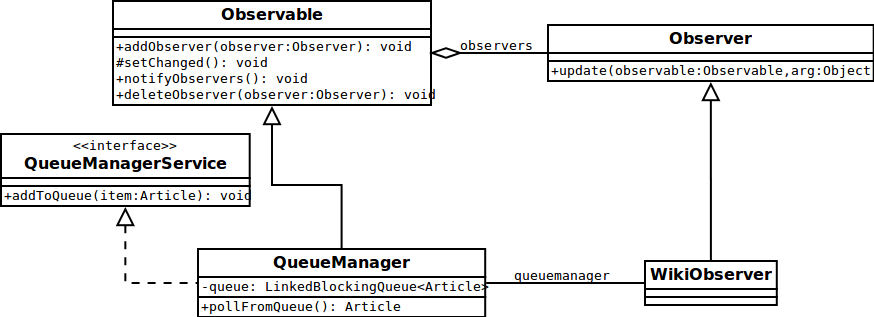
\includegraphics[scale=0.5]{img/class_parser}
\caption{Observer minta használata a Parser komponensben}
\label{fig:class_parser}
\end{figure}

Az Observer tervezési mintának köszönhetően, ha új elem kerül a queue-ba, akkor arról a \texttt{WikiObserver} értesülni fog. Mivel a cikkek feldolgozása jelentős időt vehet igénybe, azt mindenképpen külön szálakon kell megtenni. Ezt a problémát a \textit{Threadpool} tervezési mintával oldottam meg \cite{javaconcurrencyinpractice}. A \texttt{WikiObserver}-nek (\ref{fig:class_parser2}.~ábra) van egy \texttt{ThreadPool} példánya, és ha értesül a queue frissüléséről, egy új feladatot fog a \texttt{ThreadPool}-hoz hozzáadni. A ThreadPool mintának megfelelően minden feladat (\texttt{WikiWorker}) külön szálon fut. 

\begin{figure}[htp]
\centering
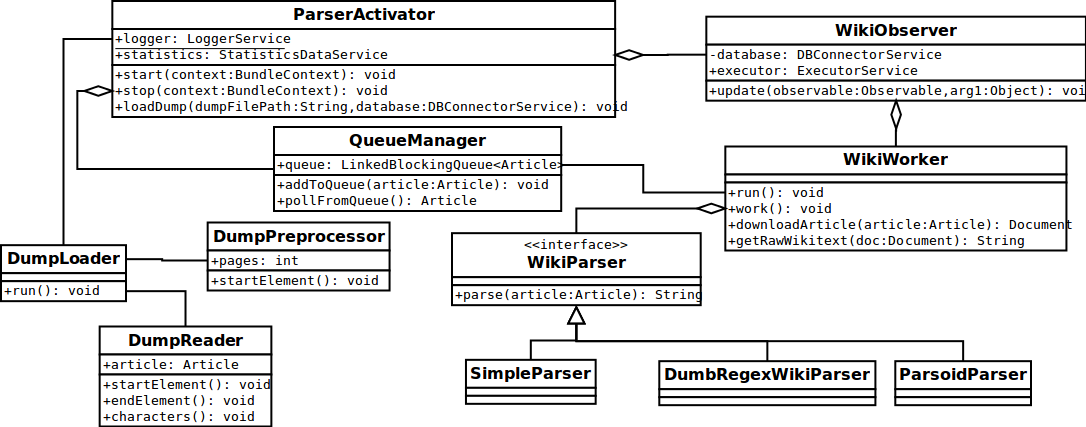
\includegraphics[scale=0.55]{img/class_parser2}
\caption{A Parser komponens osztálydiagramja}
\label{fig:class_parser2}
\end{figure}

Ebben a fázisban első lépésben először letöltődnek a hivatalos Wikipédia API-n keresztül a cikkek tartalmai. A Wikipédia a felhasználók számára könnyebben szerkeszthető \textit{Wikitext} formátumban teszi elérhetővé a cikkek tartalmait. A Wikitext egy egyszerű, könnyen használható jelölőnyelv, mely egyértelműen leképezhető a HTML formátumra, így könnyen készíthetőek vele webes tartalmak.

Azonban ez a Wikitext formátum kevésbé jól feldolgozható, mint például a HTML formátum, így a cikkek szövegét HTML formába célszerű alakítani. A második fázisban tehát ez az átalakítás történik meg, ha nem volt még újabb verziójú változat az adott cikkből az adatbázisban. Ehhez ún. parser-eket lehet használni, melyből három felcserélhető, különböző előnyökkel és hátrányokkal rendelkező változat is került a feldolgozóláncba.

\begin{itemize}
	\item Sztakipedia parser \cite{sztakipediaparser}: Könnyen testreszabható és általános célú program, mely a MediaWiki Wikitext formátumról tud HTML formátumra átalakítani. Oláh Tibor BME mérnök informatikus hallgató 2011. évi gyakornoki munkája az MTA SZTAKI-ban. Ez a program egy könnyen kiterjeszthető \textit{Visitor} tervezési mintára alapuló szoftver, mely önálló csomagként is használható a jól felépített API-nak köszönhetően. Használata nagyon egyszerű, használható kimenetet állít elő és sebesség szempontjából is jól teljesít, viszont nagyon nagy méretű fájloknál, például egy teljes Wikipédia dump feldolgozásánál rendkívül sok memóriát használ. Ennek a tulajdonságnak köszönhetően, csak on-the-fly feldolgozás során használható eredményesen ez a parser.
	
	\item DumbRegexWikiParser parser: A végletekig leegyszerűsített MediaWiki Wikitext átalakító Héder Mihály 2011. évi munkája, mely egy SAX parser implementáció. Az állapotgépes Wikitext feldolgozásnak köszönhetően nem fogyaszt annyi memóriát, mint a Sztakipedia parser, sebesség szempontjából még gyorsabb is az előzőnél, viszont kevésbé használható kimenetet produkál.
	
	\item Parsoid parser: Ez az átalakító a WikiMedia Alapítvány által, 2011 óta fejlesztett és használt szoftver, mely a Wikitext egy ekvivalens HTML / RDFa kimenetét készíti el, mely automatikus feldolgozásra rendkívül jól használható. Az RDFa szabványban meghatározott attribútumokkal kiegészített HTML kód, sokkal nagyobb jelentéstartalommal bír, mint az alap HTML dokumentum, így a szöveg sokkal jobb lesz további felhasználhatóság szempontjából. A Parsoid egy NodeJS-ben írt szoftver, így felhasználása Java nyelvű alkalmazásokban sokkal nehezebb, mint a korábbi parser megoldásoké, viszont kimenete a célnak leginkább megfelelő, így ez lett az ajánlott átalakító mechanizmus a feldolgozóláncban.
\end{itemize}

Végül a cikk feldolgozásának utolsó, harmadik fázisában eltárolódik a cikk a rendszer adatbázisában. Ebbe a fázisba akkor ér el a feldolgozás, ha nem volt újabb verziójú változat az adott cikkből még az adatbázisban. A verziók meghatározása a cikkek verziószáma alapján történik. Ha régebbi verziószámú cikk már volt az adatbázisban, akkor azt csak frissíteni kell, ellenkező esetben az adott cikknek még semmilyen változata nem létezik az adatbázisban, így azt újonnan kell beszúrni.

Ennél a komponensnél a  megfigyelhetőséget naplózással és különféle metrikák lekérdezhetőségével oldottam meg. A \texttt{ParserActivator} indulásakor a \texttt{Logger} komponens (\ref{sec:loggerbundle}.~alfejezet), és a \texttt{Statistics} komponens (\ref{sec:statisticsbundle}.~alfejezet) referenciáját is megszerzi.

\subsection{Wikipédia dump feldolgozás}
\label{sub:dumpprocessing}

A feldolgozólánc indulásakor, lehetőség van az éppen frissülő cikkek on-the-fly feldolgozásán és adatbázisba való eltárolásán túl a már korábban a Wikipédián elérhető cikkek eltárolására is, melynek forrása a havonta frissülő Wikipédia állománya, amit XML formátumban tesznek elérhetővé.

A dump feldolgozása nagyon hasonlít az on-the-fly feldolgozáshoz, szintén egy \texttt{WikiObserver} példány irányítja a feldolgozást és egy \texttt{QueueManager}-t használ a cikkek ideiglenes eltárolásához. A hatalmas méretű (2013. októberében 44 GB) XML fájl, melyben a Wikipédián olvasható cikkek vannak eltárolva, a feldolgozás során először egy előfeldolgozáson megy keresztül, ahol gyorsan néhány statisztikai adatot gyűjt a program az adatbázismentésről. Ilyen statisztikai adat például a dump-ban lévő cikkek száma, így követhető a feldolgozás állapota a tényleges beolvasás során. Ekkora méretű fájlt csak valamilyen állapotgép alapú megoldással lehet feldolgozni, ilyen például \textit{SAX Parser} (Simple API for XML). A parser a megszerzett cikket egy queue-ban tárolja el, ahonnan a \texttt{WikiObserver} kiszedi, annak szövegét átalakítja HTML formátumra és eltárolja az adatbázisban.

% subsection dumpprocessing (end)

% section parserbundle (end)

\section{DatabaseConnector bundle}
\label{sec:dbconnectorbundle}
    
Ebben a komponensben lesz az adatbázisban eltárolva a Parser komponens által feldolgozott minden cikk. Feladatai közé tartoznak tehát az adatbáziskezeléssel kapcsolatos műveletek elfedése más rétegek elől: cikkek eltárolása, frissítése, törlése és különböző szempontok alapján való keresés a cikkek között, azaz a CRUD műveletek (create, read, update, delete). A feldolgozóláncra alapuló további rétegek számára -- melyet külső fejlesztők (a rendszer felhasználói) készítenek -- ez a komponens egy csatlakozási pont, így kiajánlott szolgáltatását alacsonyabb és magasabb rétegben lévő komponensek is használhatják, az adatbázissal való kommunikáció teljesen el van fedve előlük.

\begin{figure}[htp]
\centering
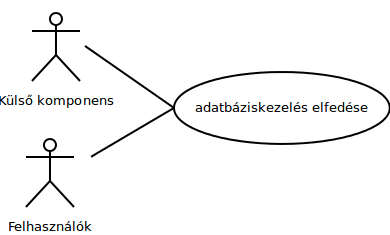
\includegraphics[scale=0.6]{img/usecase_dbconnector}
\caption{A DBConnector használati esetei}
\label{fig:usecase_dbconnector}
\end{figure}

A fenti use case-ek csak általánosan fogalmazzák meg a komponenssel kapcsolatos elvárásokat. Az egyes feldolgozóláncra alapuló komponensek további követelményeket is támaszthatnak a komponens iránt, például különböző szempontok alapján való keresés.

\begin{figure}[htp]
\centering
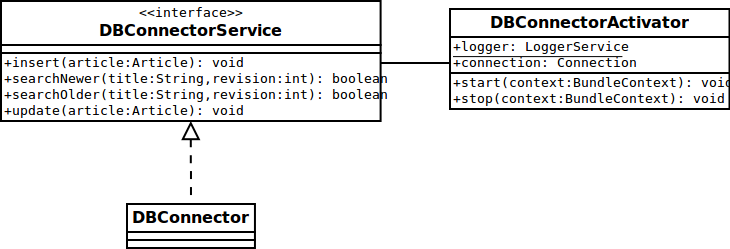
\includegraphics[scale=0.55]{img/class_dbconnector}
\caption{A DBConnector komponens osztálydiagramja}
\label{fig:}
\end{figure}

A komponens indulásakor (\texttt{DBConnectorActivator} osztály \texttt{.start()} metódusa), olyan állapotba hozza az adatbázist, hogy az később képessé váljon a fenti feladatokra, valamint egy OSGi szolgáltatást kell kiajánlani, amin keresztül a többi komponens kommunikálhat a DBConnector-ral.

% section dbconnectorbundle (end)

\section{Database}
\label{sec:db}

Az adatbázis komponens alapjául szolgáló adatbázis szoftver kiválasztását a WikiBot komponenshez hasonlóan egy rövidebb előkutatás előzte meg. Fő szempont volt, hogy nagy teljesítményű, gyors és lehetőleg az OSGi keretrendszerrel könnyen integrálható legyen a választott adatbázis megoldás. Két különböző adatbázis lehetőséget vizsgáltam meg, és a tapasztalatok alapján választottam ki a legmegfelelőbbet.

\begin{enumerate}
	\item Prevayler: Egy nagyon egyszerű és gyors adatbázis, melynek lényege, hogy minden objektumot egyszerű Java objektumokként (POJO) tartsunk a memóriában, és a tranzakciókat naplózzuk, az adatbázis pedig a használó programba beágyazottan fut. A tárolandó objektumokra egyetlen megkötés, hogy implementálják a \texttt{Serializable} interfészt, és a műveleteket is szerializálható objektumok reprezentálják. A műveleteket a Prevayler naplózza, és időnként teljes mentést (\textit{snapshot}) készít az adatbázisról, így egy rollback esetén a snapshot-ot visszaállítja és lefuttatja még a szükséges tranzakciókat.
	
Felépítéséből adódóan sokkal gyorsabb mint bármelyik RDBMS, viszont OSGi környezetben a használata egyelőre nem megoldott. A probléma oka, hogy minden OSGi komponensnek saját classloader-e van, így osztályok dinamikus betöltése, például szerializációval nem lehetséges az OSGi programokban \cite{hall04osgi}. A megoldás lehetne új \texttt{BundleClassLoader} implementálása, azonban ez a Prevayler használatának egyszerűségét rontaná el, így inkább másik megoldást választottam.

    \item H2DB: Az összegyűjtött tapasztalatok alapján arra jutottam, hogy OSGi környezetben kevésbé érdemes beágyazott adatbázist választani, ha több komponens között is meg kell oldani a kommunikációt, hiszen belső működésüket tekintve ezen adatbázisok szinte mindig használnak valamilyen szerializációs eljárást.

    A H2DB egy objektum relációs adatbázis, mely tud beágyazott és kliens-szerver módban is működni. A készítők teljesítménytesztjei alapján gyorsabb a legtöbb népszerű adatbáziskezelőnél (HSQLDB, Derby, MySQL, PostgreSQL), valamint tervezésekor megpróbálták a HSQLDB és a Derby adatbáziskezelők előnyeit is egyesíteni benne.

A H2DB további előnyei még, hogy nem szükséges telepíteni, teljes egészében Java nyelven íródott és például Java nyelvű tárolt eljárásokkal is kiegészíthetjük funkcióit. Az eddig felsorolt pozitív tulajdonságok miatt esett a választásom a H2DB-re, bár igaz, hogy beágyazott módban OSGi-al nem használható effektíven, csak úgy, mint a Prevayler. A H2DB szerver módban is használható, így JDBC adatbázishozzáférési API-val lehet kapcsolódni hozzá. A szerver módban való futtatás előnye, hogy sokkal kisebb a csatolás az adatbázissal, így például a DBConnector komponensben, ha a JDBC API-t használjuk, az adatbázis könnyen lecserélhető a rendszerben másik adatbázis megoldásra.

\end{enumerate}

\begin{figure}[htp]
\centering
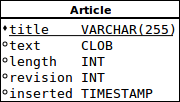
\includegraphics[scale=0.8]{img/database_article}
\caption{A tervezett adatbázis Article táblája}
\label{fig:database_article}
\end{figure}

Az adatbázis kiválasztása után, az adatbázis tábláinak megtervezése következett. Az egyszerű specifikáció miatt egyed kapcsolat diagram rajzolására nincs szükség, hiszen egyetlen egyed van az adatbázisban, mely a cikk reprezentációja (\texttt{Article}). A Wikipediában minden cikket annak címe azonosítja (\ref{fig:database_article}.~ábra), nem lehet két azonos című, de különböző cikk. Így elsődleges kulcs a cím (title) lesz, további szükséges attribútumok a szöveg (text), szöveg hossza (length), szöveg verziószáma (revision), illetve a beillesztés dátuma (inserted).

A rendszerben természetesen további adatbázisok, táblák is lehetnek, amelyeket a kutatómodulok hozhatnak létre. Ezek a kutatómodulok a rendszer által előfeldolgozott Article példányokat elemzik tovább. A DatabaseConnector komponens könnyen kiegészíthető, hogy a kutatómodulok igényeit teljesítse, azonban ez már nem az én feladatom volt.

% section db (end)

\section{Logger bundle}
\label{sec:loggerbundle}

Ha a rendszer állapotait meg akarjuk figyelni, illetve szeretnénk, ha jelezné a hibákat, mindenképpen érdemes az alkalmazást felügyeletre tervezni. Az egyik ilyen lehetőség a naplózás, mely ennek a komponensnek a fő feladata (\ref{fig:usecase_logger}.~ábra).

\begin{figure}[htp]
\centering
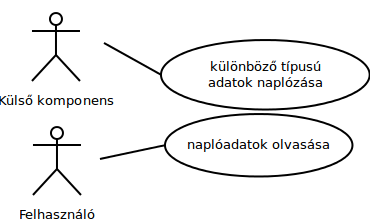
\includegraphics[scale=0.6]{img/usecase_logger}
\caption{A Logger komponens használati esetei}
\label{fig:usecase_logger}
\end{figure}

Első lépésben meg kell tervezni a rendszer felügyeleti modelljét, mely egy állapotgép formájában ábrázolható a rendszer fontosabb állapotaival. Az állapotgép átmenetei események, az átmenetek feltételei hibalehetőségek, a tranzakciók pedig naplózást jelentenek, a használt jelölés:

\begin{equation}
	esem\acute{e}ny(argumentum) [felt\acute{e}tel] / tranzakci\acute{o}
\end{equation}

Naplózás során a rendszer eseményeit több kategóriába soroltam be súlyosság és következmények szempontjából, ezek láthatóak a \ref{tab:loglevels}.~táblázatban.

\begin{table}[htb]
\begin{center}
\begin{tabular}{|c|l|}
\hline
\multicolumn{1}{|c|}{\textbf{naplózási szint}} & \multicolumn{1}{|c|}{\textbf{rövid leírás}} \\ \hline \hline
FATAL & Súlyos hiba, amely a rendszer leállásához vezet. \\ \hline
ERROR & Súlyos hiba, azonban a rendszer működése nem feltétlenül áll meg. \\ \hline
WARN  & Esetlegesen káros hatással bíró esemény. \\ \hline
INFO  & Magasszintű információ a rendszer állapotáról. \\ \hline
DEBUG & Részletes információk a rendszer állapotáról, hibakereséshez használható. \\ \hline
TRACE & Legrészletesebb információk a rendszer állapotairól. \\
\hline
\end{tabular}
\end{center}
\caption{\label{tab:loglevels} A naplózás szintjei}
\end{table}

A fent meghatározott naplózási szinteknek megfelelő naplózási eljárásokat teljesítő komponens egy OSGi szolgáltatás lesz, mely képes a naplózást a követelményeknek megfelelően elvégezni (\ref{fig:class_logger}.~ábra).

\begin{figure}[htp]
\centering
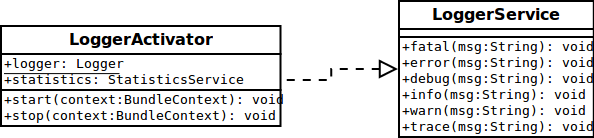
\includegraphics[scale=0.55]{img/class_logger}
\caption{A Logger komponens osztálydiagramja}
\label{fig:class_logger}
\end{figure}

% TODO: felügyeleti modellek aktualizálása

% section loggerbundle (end)

\section{Statistics bundle}
\label{sec:statisticsbundle}

Az alkalmazás felügyeletének másik lehetőségével meghatározott metrikák lekérdezésére és vizsgálatára van lehetőség. A többi komponens állapotait ennek a komponensnek a segítségével teheti elérhetővé, így a rendszer által végzett feladatról készített statisztikák megfigyelésére is van lehetősége a felhasználóknak (\ref{fig:usecase_statistics}.~ábra).

\begin{figure}[htp]
\centering
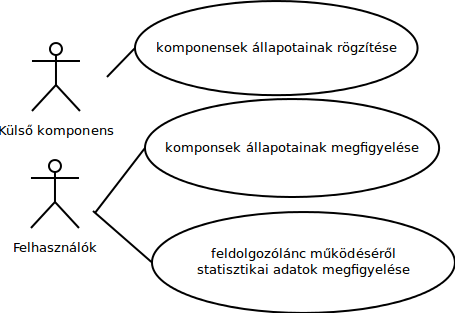
\includegraphics[scale=0.6]{img/usecase_statistics}
\caption{A Statistics komponens használati esetei}
\label{fig:usecase_statistics}
\end{figure} 

A feldolgozólánc működését átvizsgálva meghatároztam és kiválasztottam megfigyelés céljából a rendszer állapotának szempontjából fontos mérőszámokat (\ref{tab:metrics}.~táblázat).

\begin{table}[hbt]
\begin{center}
\begin{tabular}{|L{2.6cm}|L{4.5cm}|L{2cm}|L{4.7cm}|}
\hline
\textbf{metrika neve} & \textbf{metrika leírása} & \textbf{metrika mértékegy-sége} & \textbf{metrika számításának módja} \\ \hline \hline
eltárolt cikkek száma & ennyi cikk van az adatbázisban & darab & frissített cikkek száma + újonnan beillesztett cikkek száma \\ \hline
frissített cikkek száma & korábban már az adatbázisban szereplő, frissített cikkek száma & darab & ha kisebb verziószámú azonos című cikk szerepel az adatbázisban, akkor eggyel nő a száma \\ \hline
újonnan beillesztett cikkek száma & korábban még az adatbázisban nem szereplő cikkek száma & darab & ha még nem volt az adatbázisban az adott című cikk akkor eggyel nő a száma \\ \hline
nem feldolgozott cikkek száma & ennyi cikket nem dolgoztunk fel, mert újabb változat van az adatbázisban & darab & minden esetben mikor újabb verziójú cikket dolgoz fel a száma nő eggyel \\ \hline
hibák száma & FATAL, ERROR, WARN, DEBUG, INFO, TRACE üzenetek száma a naplóban & darab & log üzenet írása esetén a statisztikák száma is nő \\ \hline
queue hossza & QueueManager által karbantartott queue-ban lévő elemek száma & darab & QueueManager-be íráskor értéke nő eggyel, elem kivételekor csökken eggyel \\ \hline
feldolgozás sebessége & ennyi cikket dolgoz fel 1 perc alatt a feldolgozólánc & cikk/perc & 1 percenként elmentett cikkek számából kivonja az előző elmentett értéket \\ \hline
dolgozóparserek száma & adott nevű observerben ennyi parser dolgozik & százalék & dolgozó parserek száma / az összes elérhető parserek számával \\ \hline
dump feldolgozás állapota & ekkora százaléka lett beolvasva a dump-nak & százalék & beolvasott cikkek száma / összes cikk a dump-ban \\
\hline
\end{tabular}
\end{center}
\caption{\label{tab:metrics} A Statistics komponens által megfigyelhető metrikák}
\end{table}

Az eddigi követelmények alapján úgy tűnhet, hogy a legjobb választás a JMX (Java Management Extensions) technológia lenne a feladatra, azonban több szempont alapján sem ezt választottam. Bár később a rendszer valamilyen szintű menedzselése szükségessé válhat, mégis OSGi környezetben nem biztos, hogy a JMX a legjobb megoldás. Egyrészt a JMX nem építhető be a már korábban említett OSGi tulajdonságok miatt a rendszerbe, így egy másik implementációt a MOSGi-t (Managed OSGi) kellene használni; másrészt a MOSGi egy sokkal bonyolultabb architektúrát használ és a felhasználók számára sem annyira egyszerű a kezelése.

\begin{figure}[htp]
\centering
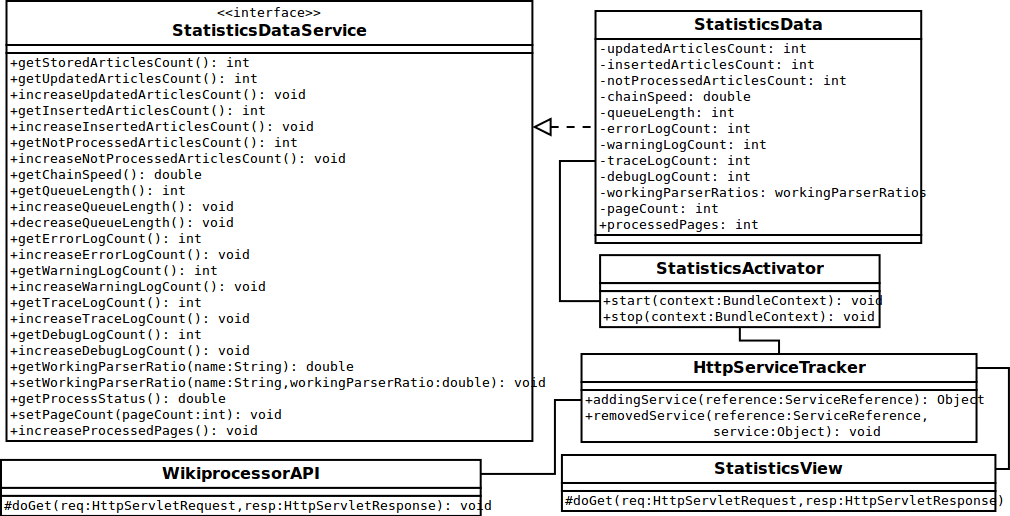
\includegraphics[scale=0.45]{img/class_statistics}
\caption{A Statistics komponens osztálydiagramja}
\label{fig:class_statistics}
\end{figure}

A fent felsorolt indokok alapján döntöttem saját menedzselő komponens fejlesztése mellett, mely egy sokkal egyszerűbb architektúrát követ, és nagyon könnyen kiegészíthető. A menedzser komponens egy OSGi szolgáltatásból áll (\texttt{StatisticsDataService} a \ref{fig:class_statistics}.~ábrán), melybe a többi komponens rögzítheti az állapotait, illetve két servlet segítségével tud kapcsolatba lépni a felhasználókkal, melyek közül az egyik JSON formátumban elérhetővé teszi a statisztikai adatokat (\texttt{WikiprocessorAPI}), a másik pedig egy HTML oldalt készít a statisztikai adatokkal (\texttt{StatisticsView}). Az elkészített HTML oldalon grafikonok készülnek el dinamikusan Javascript + Ajax segítségével, így az elkészült weboldalon friss statisztikai adatokat lehet megfigyelni folyamatosan a rendszer állapotáról és a futó folyamatokról.

A Statistics komponens többféleképpen is megszerezheti a feldolgozólánc többi komponensének állapotait. Az egyik lehetőség, hogy saját maga gyűjti az adatokat az eseményekről, a különböző komponensek feliratkoznak a kiajánlott statisztika készítő szolgáltatásra és így frissítik a metrikákra vonatkozó adatokat. Emiatt ezen komponensek (például a Parser) függeni fognak a Statistics komponenstől. Ekkor, ha a parserben lévő queue-ról is szeretnénk adatokat, az egyik lehetőség, hogy a queue minden módosulásánál tájékoztatja a statisztika készítő komponenst a megváltozásról, ez azonban overhead-del jár a queue számára. A másik megoldás, hogy a statisztika készítő komponens kéri le a queue hosszát, ha szüksége van rá, így azonban a Statistics komponens is függeni fog a Parser-től. Emiatt, ha a második lehetőséget választanánk, ami nem jár akkora overhead-del, más a Parser-nél alacsonyabb szintén lévő komponensek nem használhatnák a Statistics komponenst, hiszen a függőségek alapján az OSGi keretrendszer nem tudna előállítani olyan komponens indítási sorrendet, amelyben minden indítási függőség kielégülne (függőségi hurok alakulna ki). A megmaradt választási lehetőség tehát az, ha minden komponens folyamatosan tájékoztatja a megfigyelhető állapotairól a Statistics komponenst.

% section statisticsbundle (end)

\section{Research bundle-ök}

Ezen kutató bundle-ök tervezése nem tartozott a feladataim közé. Működésüket tekintve sokféle céljuk lehet, például mondattani elemzés, szemantikus annotálás, szó együttes előfordulás analízis (ko-okkurencia), vagy egyéb természetes nyelvi feldolgozás témakörébe eső feladat.

A kutatókomponensek dolgozhatnak direkt módon a H2DB adatbázison, vagy használhatják a kiajánlott OSGi szolgáltatásokat és akkor értesülhetnek az éppen frissülő cikkekről, megkaphatják az elkészült Article példányokat. A cikk példányokkal tetszőleges műveleteket hajthatnak végre, de fontos, hogy ne tartsák fel a rendszer működését.

A rendszer funkcióinak tesztelésekor (\ref{cha:test}.~fejezet) egy MTA SZTAKI által készített teszt kutatómodult használtam, mely a cikkekben szereplő link és kategóriahivatkozásokat és a hozzájuk köthető szöveges megjelenési formákat elemezte. További kutatómodulok fejlesztése a későbbiekben várható még, ezért a feldolgozólánc többi elemét is fel kell erre készíteni.

\label{sec:researchbundle}

% section researchbundle (end)

% chapter design (end)